\section{Methodology}
We present \plugmem, a task-agnostic plugin memory module to support long-term decision-making for LLM agents. Rather than treating past interactions as flat episodic text, \plugmem structures experience into knowledge-level representations that are more compact, generalizable, and directly relevant to downstream retrieval and reasoning.

As shown in Figure~\ref{fig:overview}, \plugmem consists of three core components: \textit{a structuring module} that standardizes heterogeneous episodic memories and induces propositional and prescriptive knowledge; \textit{a retrieval module} that selects relevant knowledge from structured memory graphs via abstraction-aware retrieval; and \textit{a reasoning module} that further adapts retrieved knowledge into actionable guidance for the base agent. In the following sections, we describe each component in detail.
\begin{figure*}[ht]
    \centering
    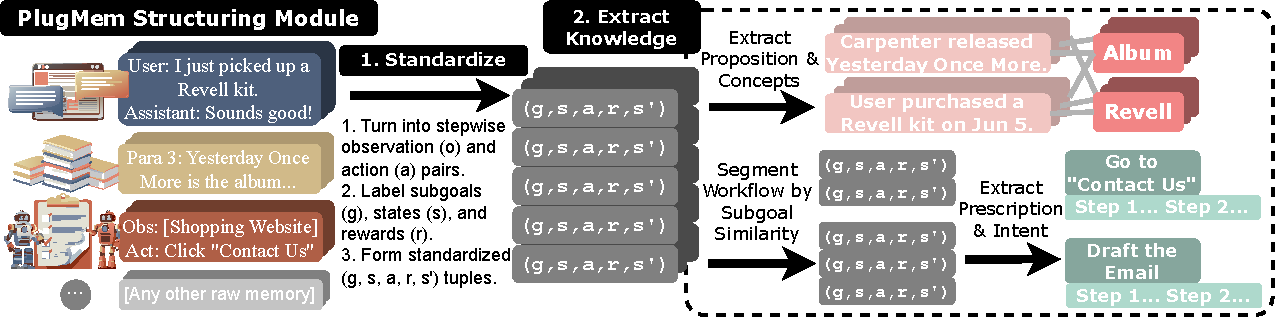
\includegraphics[width=\textwidth]{Figures/structuring_module.pdf}
    \caption{\label{fig:structuring_module}
    The structuring module in \plugmem transforms heterogeneous memory into a formalized knowledge-dense memory graph.
    }
\end{figure*}
\subsection{Structuring Module}
\label{subsec:structuring}
\begin{table*}[ht]
\centering
\caption{\textbf{Mapping Memory Properties to Graph Architecture.} We analyze long-term memory properties to derive our memory graph design. The main rationale is \textbf{aligning memory structure with the granularity at which knowledge is acquired, stored, and reasoned over}, reflected here as ensuring core nodes represent complete, self-contained, and verifiable \textbf{knowledge blocks} (Propositions/Prescriptions), thus improving the efficiency and fidelity of downstream graph operations.}
\label{tab:memory_rationale}
\resizebox{\textwidth}{!}{%
\begin{tabular}{@{}l l l l@{}}
\toprule
\textbf{Memory Type} & \textbf{Nature \& Description} & \textbf{Knowledge-Dense Unit} & \textbf{Subgraph Structuring Logic} \\ 
\midrule

\textbf{Semantic} & \begin{tabular}[c]{@{}l@{}}\textbf{Declarative \& Static} \\ Context-independent concepts, \\ facts, and world knowledge.\end{tabular} & \begin{tabular}[c]{@{}l@{}}\textbf{The Proposition (Fact Block)} \\ A complete statement conveying \\ verifiable truth.\end{tabular} & \begin{tabular}[c]{@{}l@{}}\textbf{Concept-Centric Semantic Mem Structuring} \\ \textit{Logic:} Concepts acts as lightweight indices \\ pointing to heavy Proposition payloads. \\ \textit{Structure:} \texttt{Concept} $\xleftarrow{mentions}$ \texttt{Proposition}\end{tabular} \\ 
\midrule

\textbf{Procedural} & \begin{tabular}[c]{@{}l@{}}\textbf{Executive \& Goal-Oriented} \\ Dynamic ``how-to'' knowledge \\ for problem solving.\end{tabular} & \begin{tabular}[c]{@{}l@{}}\textbf{The Prescription (Workflow Block)} \\ A full action sequence to execute a\\ complex task.\end{tabular} & \begin{tabular}[c]{@{}l@{}}\textbf{Intent-Centric Procedural Mem Structuring} \\ \textit{Logic:} Intents (User Goals) serve as keys to \\ find holistic Solution blocks. \\ \textit{Structure:} \texttt{Intent} $\xleftarrow{solves}$ \texttt{Prescription}\end{tabular} \\ 
\midrule

\textbf{Episodic} & \begin{tabular}[c]{@{}l@{}}\textbf{Autobiographical \& Linear} \\ Raw record of past interactions \\ and observations. Large volume.\end{tabular} & \begin{tabular}[c]{@{}l@{}}\textbf{The Source Trace (Event Window)} \\ A trajectory segment for grounding and \\ verification.\end{tabular} & \begin{tabular}[c]{@{}l@{}}\textbf{Episodic Mem as the Anchor} \\ \textit{Logic:} Episodic acts as the ``ground truth'' layer \\ validating the abstract knowledge graphs. \\ \textit{Structure:} \texttt{Knowledge} $\xleftarrow{proves}$ \texttt{Source}\end{tabular} \\

\bottomrule
\end{tabular}%
}
\end{table*}
As shown in Figure~\ref{fig:structuring_module}, the structuring module serves as the foundation of \plugmem by transforming raw episodic experience, such as dialogue turns, document snippets, or episodic trajectories, into knowledge representations that are reusable, compact, and aligned with agent decision-making. Specifically, we structure memory to reflect the role different information plays in reasoning and action selection.


Our design is guided by three principles motivated by cognitive theories of human memory. First, episodic memory captures concrete interaction traces and serves primarily as verifiable evidence rather than directly actionable knowledge. Second, decision-relevant information is most effectively represented at the knowledge level, where semantic memory encodes factual propositions (``knowing that'') and procedural memory encodes reusable strategies (``knowing how''). Third, effective long-term memory requires separating knowledge abstraction from task-specific execution details, enabling memory to generalize across heterogeneous environments. These principles imply that different memory types should be represented using structural units and organization logics aligned with their properties. Table~\ref{tab:memory_rationale} summarizes how episodic, semantic, and procedural memories are mapped to corresponding graph units and structuring mechanisms, reflecting their functional roles in abstraction, retrieval, and verification.

Building on this design, the structuring module operationalizes memory abstraction in two stages: \textit{i)} standardizing heterogeneous interaction traces into a unified episodic representation, and \textit{ii)} inducing propositional and prescriptive knowledge that can be independently indexed and reused across tasks. We describe each stage as follows.

\begin{figure*}[ht]
    \centering
    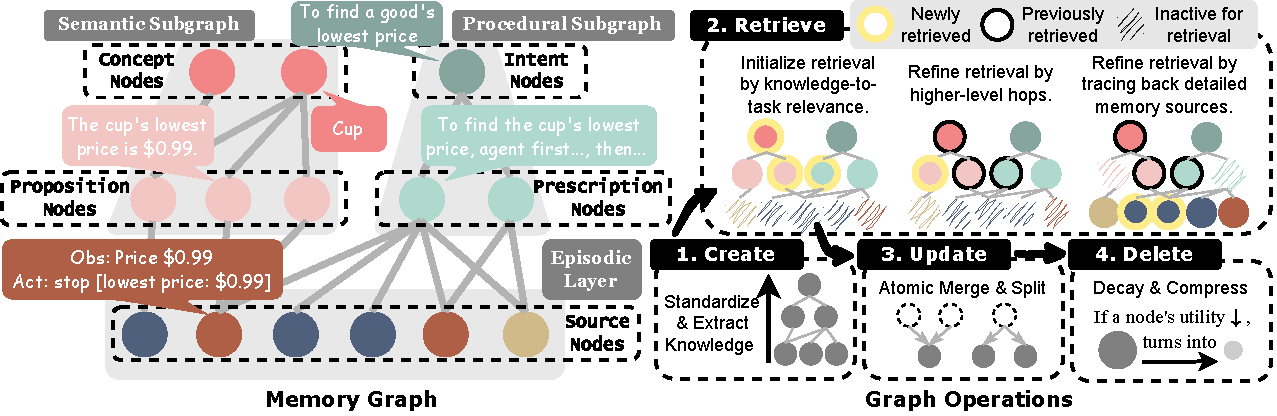
\includegraphics[width=\textwidth]{Figures/memory_graph.pdf}
    \caption{\label{fig:memory_graph}
    \plugmem's knowledge-centric memory graph design and the standard graph operations it supports.
    }
\end{figure*}
\subsubsection{Standardize}
\label{subsubsec:standardize}

Episodic memory constitutes the fundamental substrate from which semantic and procedural memories are derived~\citep{Tulving1972EpisodicSemantic}. 
For agents, episodic memories originate from heterogeneous sources, including user--agent interactions~\citep{wu2024longmemeval}, factual documents~\citep{yang2018hotpotqadatasetdiverseexplainable}, and action trajectories in complex environments~\citep{zhou2024webarenarealisticwebenvironment}. 
This heterogeneity motivates a unified, task-agnostic representation that can support downstream knowledge induction.

\paragraph{Episodic Formalization.}
We represent a raw interaction trace as a sequence of observation-action pairs:
\[
\tau = [(o_t, a_t)]_{t=1}^{T}
\]
While episodic memory is widely used in agent systems, its internal structure is often treated as unstructured text.
In contrast, we explicitly formalize episodic memory at the step level by mapping each interaction into a structured tuple. Specifically, each pair $(o_t, a_t)$ is standardized as:
\[
e_t = (o_t, s_t, a_t, r_t, g_t)
\]
where $s_t$ denotes the agent state at time $t$, $g_t$ denotes the subgoal associated with executing $a_t$, and $r_t$ denotes the reward of the action with respect to $g_t$.

The state $s_t$ is derived from $(s_{t-1}, a_{t-1}, o_t)$ via LLM-based information extraction.
Both $g_t$ and $r_t$ are annotated by an LLM conditioned on the task instruction and local interaction context.
Aggregating all standardized steps yields an episodic memory sequence
\[
M_{\text{epi}} = [e_t]_{t=1}^{T}
\]
Implementation details of episodic standardization, including the prompt template, are provided in Appendix~\ref{app:implementation_standardize_episodic}.


\subsubsection{Extract Knowledge}
\label{subsubsec:extract}

We focus this section on the design of the knowledge extraction and organization process.
Implementation details, including model choices, parameter settings, and prompt configurations, are deferred to Appendix~\ref{app:implementation_extract_knowledge}.

Given standardized episodic memory $M_{\text{epi}}$, we induce two complementary forms of long-term memory: semantic memory and procedural memory. 
Both are extracted from episodic experience and organized as structured memory graphs with provenance.

\paragraph{Semantic Memory.}
The semantic memory module extracts and stores factual knowledge from episodic memory to support later retrieval.
Given an episodic unit $e_t$, the module uses an LLM to extract a set of atomic propositions that describe salient facts implied by the interaction.
Each proposition is accompanied by a set of associated concepts, which serve as semantic tags for indexing.
For example, a proposition may be:
\emph{``Tam Sventon, known in Swedish as Ture Sventon, is a fictional private detective based in Stockholm.''}
The associated concept set is \{\emph{Tam Sventon, fictional private detective, Stockholm}\}.
To ensure extraction quality, we apply several constraints during LLM extraction, including coreference resolution, proposition deduplication, and length control.

The extracted propositions and concepts are stored in a semantic graph $G^{S}$.
Each proposition and concept is instantiated as a node with a cached dense embedding.
Two types of edges are constructed:
\textit{i)} \emph{membership} edges linking propositions to their associated concepts, and
\textit{ii)} \emph{provenance} edges linking propositions to their source episodic units in the episodic graph $G^{E}$.
This design allows retrieved semantic knowledge to be traced back to its originating experience.



\paragraph{Procedural Memory.}
The procedural memory module extracts reusable action strategies from episodic trajectories to support future decision making.
Given an episodic sequence $M_{\text{epi}}$, the module first segments the trajectory into coherent sub-trajectories by detecting boundaries where the similarity between adjacent subgoals $g_{t-1}$ and $g_t$ falls below a predefined threshold.
For each trajectory segment, the module uses an LLM to induce a compact \emph{(intent, prescription)} pair.
The intent represents the objective pursued within the segment, while the prescription specifies an environment-agnostic action workflow that captures the key steps and cause-effect patterns required for successful execution.
An example prescription is:
\emph{``To identify the lowest price of an item, search for the item using the search bar, sort the results by price, and verify the minimum across variants.''}
To enable quality-aware reuse, each induced prescription is assigned a scalar \emph{return} score.
The score is obtained using an LLM-based evaluator that assesses whether the intent is achieved and how well the prescription is executed.

The extracted intents and prescriptions are stored in a procedural memory graph $G^{P}$.
Each intent and prescription is instantiated as a node with a cached dense embedding.
Edges in $G^{P}$ encode two types of relations.
First, \emph{hierarchical} edges link each high-level intent node to its associated low-level prescription nodes.
Second, \emph{provenance} edges link prescription nodes to their originating episodic units in the episodic graph $G^{E}$, enabling procedural knowledge to be traced back to concrete interaction experience.


\subsection{Retrieval Module}
\label{subsec:retrieval}

This section describes the high-level retrieval process over semantic and procedural memory graphs.
Detailed prompt templates, the step-by-step retrieval algorithm, and more technical details are deferred to Appendix~\ref{app:implementation_retrieval}.

In the structuring stage, \plugmem constructs three interlinked memory graphs: an episodic graph $G^{E}$, a semantic graph $G^{S}$, and a procedural graph $G^{P}$.
Both $G^{S}$ and $G^{P}$ maintain explicit provenance links to $G^{E}$, enabling verifiable grounding of retrieved knowledge and experience.
Figure~\ref{fig:memory_graph} illustrates the overall memory organization.

Given a task description or query $Q$, an LLM-based retriever first determines which memory types to emphasize: \emph{episodic}, \emph{semantic}, or \emph{procedural}.
Retrieval primarily operates over $G^{S}$ and $G^{P}$ using an abstraction-specificity interleaving strategy.
When episodic memory is prioritized, the same retrieval process (as will be introduced below) is applied, but the system ultimately returns provenance-linked episodic nodes in $G^{E}$.

Retrieval begins by encoding $Q$ into an embedding $q$ and scoring it against all low-level nodes (i.e., proposition or prescription nodes) to initialize a candidate set $C_0$.
At hop $t$, the retriever conditions on $(Q, C_t)$ to generate an abstract query $q^{a}_{t}$.
For $G^{S}$, $q^{a}_{t}$ is represented as a set of concepts, while for $G^{P}$ it is represented as a set of intents.

The abstract query $q^{a}_{t}$ is matched against high-level (i.e., concept or intent nodes) nodes, which act as routing signals to activate adjacent low-level nodes that are added to $C_{t+1}$.
Only low-level nodes are retained as candidates, while high-level nodes serve exclusively as intermediate traversal signals.
When $|C_t|$ exceeds a predefined budget (e.g., top-$K$), candidates are re-ranked and pruned based on relevance and importance. This multi-hop retrieval process iterates until sufficient evidence is accumulated or a maximum hop limit is reached.



\subsection{Reasoning Module}
\label{subsec:reasoning}

The reasoning module is a \emph{test-time running module} that transforms retrieved memory into immediately actionable guidance for the playing agent.
In many cases, retrieved memory may contain multiple overlapping or verbose descriptions of past interactions that are individually relevant but collectively redundant for the current decision.
The reasoning module leverages the LLM to aggregate and condense such information into a compact, task-aligned representation, distilling the shared signal across messages into a single actionable summary. More technical details are included in Appendix~\ref{app:implementation_reasoning}.


\subsection{Summary and Supported Operations}
\label{subsec:summary}
As shown in Figure~\ref{fig:structuring_module} and~\ref{fig:memory_graph}, starting from raw agent interactions, \plugmem standardizes episodic memory, extracts semantic and procedural knowledge, organizes them into structured memory graphs, and enables retrieval and reasoning over stored experience to support downstream decision making.
At the system level, \plugmem supports a set of basic memory graph operations, including: \textit{i)} \emph{create}, which inserts newly observed episodic experience into structured memory, \textit{ii)} \emph{retrieve}, which retrieves relevant semantic, procedural, or episodic memory given a task or query, \textit{iii)} \emph{update}, which revises existing memory entries when new evidence becomes available, and \textit{iv)} \emph{delete}, which removes obsolete or low-utility memory.

The benchmark evaluations in the main paper primarily evaluate the \emph{create} and \emph{retrieve} operations.
Additional experiments evaluating the effectiveness of the \emph{update} and \emph{delete} operations are provided in Appendix~\ref{app:full_operation}.
